\documentclass[spanish,12pt,letterpapper]{article}
\usepackage{babel}
\usepackage[utf8]{inputenc}
\usepackage{graphicx}
\begin{document}
	\begin{titlepage}
		\begin{center}
			
\includegraphics[width=0.6\textwidth]{../logoUnADM}~\\[1cm] 
			\textsc{Universidad Abierta y a Distancia de México}\\[0.8cm]
			\textsc{Desarrollo de Software}\\[1.8cm]
			
			\textbf{ \Large Evidencia de aprendizaje. Organización de información para una base de datos }\\[3cm]
			
			Diego Antonio Plascencia Lara\\ ES1421004131 \\[0.4cm]
			Facilitador(a): CESAR ALEXIE CHAN PUC  \\
			Materia: Diseño de Bases de Datos\\
			Grupo: DS-DDBD-1601-B1-003 \\
			Unidad: III \\
			
			\vfill México D.F\\{\today}
			
		\end{center}
	\end{titlepage}
	
	\section{Planteamiento del Problema}	
	''Se requiere desarrollar un sistema de base de datos para la administración de un establecimiento especializado en computación. El establecimiento dispone varios productos que se pueden vender a los clientes.\\

De cada producto informático se desea registrar  el código\_producto, descripción, precio y número de existencias. De cada cliente se desea guardar el código\_cliente, nombre, apellidos, dirección y número de teléfono. Un cliente puede comprar varios productos en el establecimiento y un mismo producto puede ser comprado por varios clientes. Cada vez que se compra un artículo quedará registrada la compra en la base de datos junto con la fecha en la que se ha comprado el artículo. El establecimiento tiene contactos con varios proveedores que son los que suministran los productos. Un mismo producto puede ser suministrado por varios proveedores. De cada proveedor se desea guardar el código\_proveedor, nombre, apellidos, dirección, provincia y número de teléfono``\\
	
	\subsection{Puntos a tratar}
	\begin{itemize}
	\subsubsection{Identificación de un SGBD}
	\item Incluye la problemática a resolver.
	\item Indica el SGBD a utilizar y justifica la elección.
	\item Menciona las entidades, atributos y relaciones de la problemática a resolver.
	\subsubsection{Modelo Relacional y Orientado a Objetos}
	\item Elabora el diagrama del modelo entidad-relación del caso a resolver.
	\item Elabora el diagrama del modelo orientado a objetos del caso a resolver.
	\item Explique las relaciones del caso a resolver.
	\subsubsection{Utilización del Gestor de Base de Datos}
	\item Crea la base de datos en el SGBD que instalaste y recuerda que debes capturar la pantalla de cada paso para poder ser evaluado en esta sección.
	\item Crea las tablas de tu modelo relacional con instrucciones SQL. Y recuerda capturar pantallas de cada paso para poder ser evaluado en esta sección.
	\item Ingresa al menos cinco datos en cada tabla para crear cinco sentencias instrucciones SQL. Y recuerda capturar las pantallas de cada paso para poder ser evaluado en esta sección.
	\item Mostrar la información de la tabla Clientes. Y recuerda capturar las pantallas de cada paso para poder ser evaluado en esta sección.
	\item Mostrar los artículos comprados por los clientes con los datos completos. Y recuerda capturar las pantallas de cada paso para poder ser evaluado en esta sección.
	\item Mostrar los proveedores de cada producto. Y recuerda capturar las pantallas de cada paso para poder ser evaluado en esta sección.
	\item Explica qué tipo de organizador físico integrarías en el
	\subsubsection{Conclusiones}
	\item Explica la forma de organizar la información y su importancia en el diseño de bases de datos.
	\item Justifica el tipo de organizador físico seleccionado.
	\item Redacta las principales dudas y obstáculos que identificó al realizar la actividad.
	\end{itemize}
	\pagebreak
	
	\section{Identificación SGBD}
	Para este ejercicio también utilizare PostgreSQL, por su licencia, que es un DBMS libre, de código abierto con licencia tipo MIT, sobre MySQL pues esta tiene licencia GPL y cuenta con licencias comerciales (requieren remuneración a Oracle); por su flexibilidad, no solo en cuanto a el código (cuenta con una librería en c), sino también por la flexibilidad en cuanto a la implementación pues permite trabajar como si fuera un RDBMS o NoSQL, e incluso un hibrido.\\
	
	\subsection{Entidades y atributos}
	
		\begin{center}
	\begin{tabular}{| p{4cm} | p{4cm} |}
	\hline
	
	\textbf{Entidad} & \textbf{Atributos}\\
	\hline
	Product & id \linebreak description \linebreak price \linebreak stock\\
	\hline
	Cliente & id \linebreak first\_name \linebreak last\_name \linebreak address \linebreak tel\\
	\hline
	Order & date \\
	\hline
	Provider & id \linebreak first\_name \linebreak last\_name \linebreak address \linebreak city \linebreak tel\\
	\hline	
	\end{tabular}
	\end{center}
	
	\subsection{Relaciones}	
	En este ejercicio hay 3 relaciones \textbf{1:N} entre \textbf{Customer-Orders}, \textbf{Product-Orders} y \textbf{Product-Providers}. Pues se menciona que \textit{``Un cliente puede comprar varios productos en el establecimiento y un mismo producto puede ser comprado por varios clientes.''} esto es una relación N:M entre Customer-Product, pero también se menciona el verbo y una entidad ''Order`` por lo que la relación pasa a ser entre y a través de Order. También se menciona \textit{``Un mismo producto puede ser suministrado por varios proveedores.''} es decir la relación 1:N entre un Product y sus Providers.
	
	\section{Modelo Relacional y Orientado a Objetos}
	\subsection{Relacional}
	\begin{center}
	\includegraphics[width=0.8\textwidth]{./relacional2}~\\[1cm] 
	\end{center}	
	
	\subsection{Orientado a Objetos}
	\begin{center}
	\includegraphics[width=0.8\textwidth]{./objetos}~\\[1cm] 
	\end{center}
	
	\section{SGBD}
	\subsection{Base de datos y tablas}
	\begin{center}
	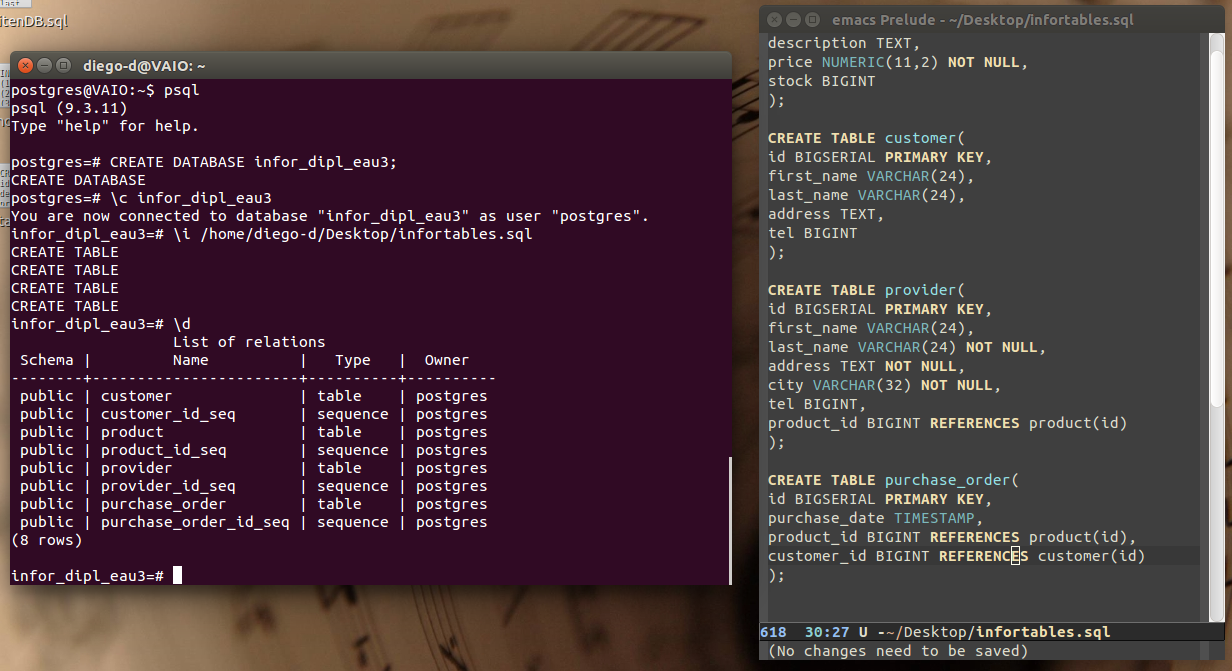
\includegraphics[width=1\textwidth]{./tables}~\\[1cm] 
	\end{center}	
	
	\subsection{Registros}
	\begin{center}
	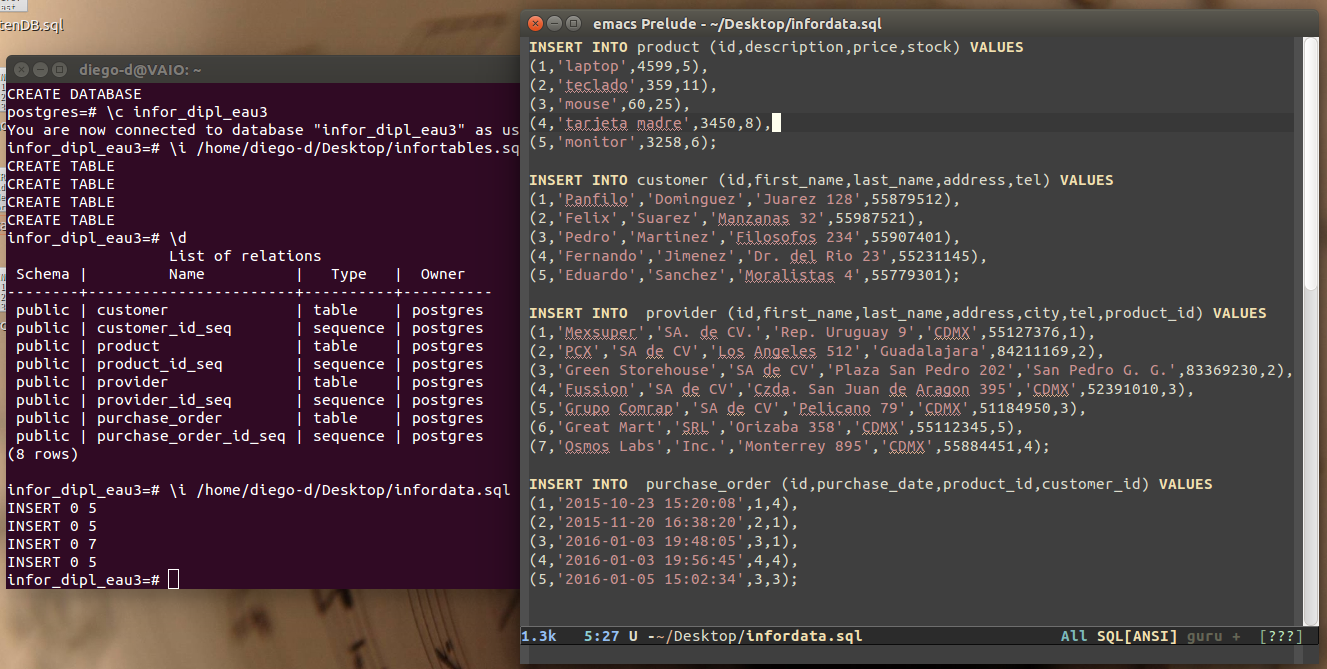
\includegraphics[width=1\textwidth]{./inserts}~\\[1cm] 
	\end{center}	
	
	\subsection{Información de los clientes}
	\begin{center}
	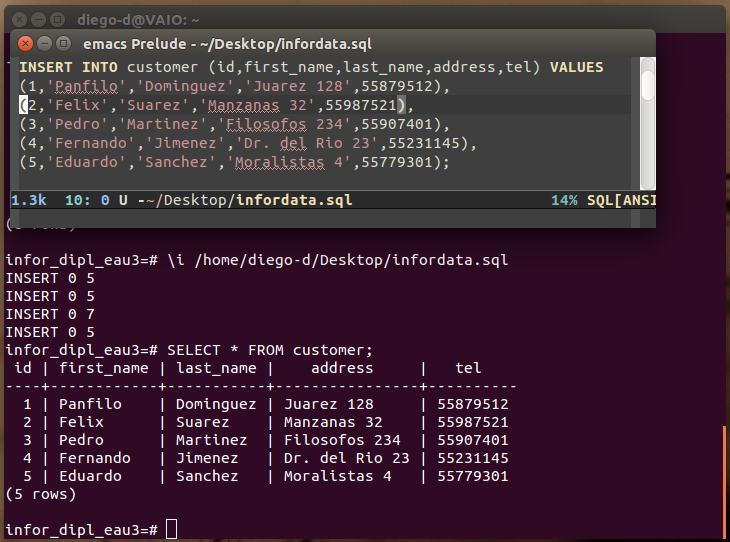
\includegraphics[width=1\textwidth]{./customers}~\\[1cm] 
	\end{center}	
	
	\subsection{Clientes y sus productos}
	\begin{center}
	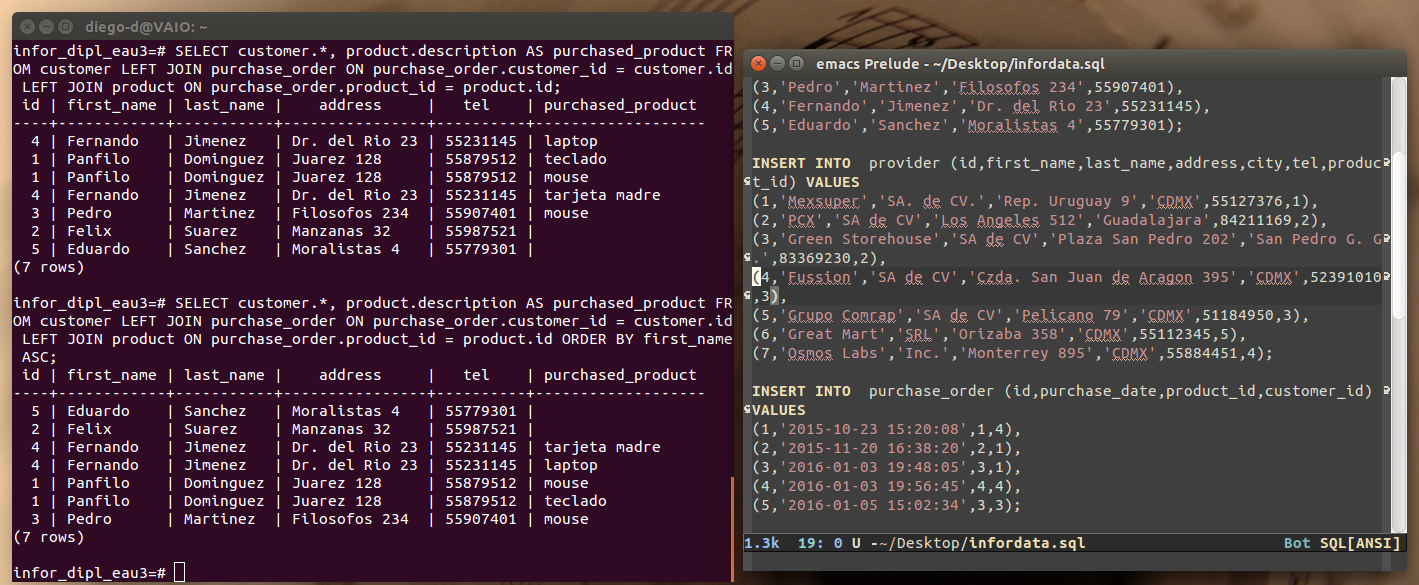
\includegraphics[width=1\textwidth]{./customerproducts}~\\[1cm] 
	\end{center}	
	
	\subsection{Productos y sus proveedores}
	\begin{center}
	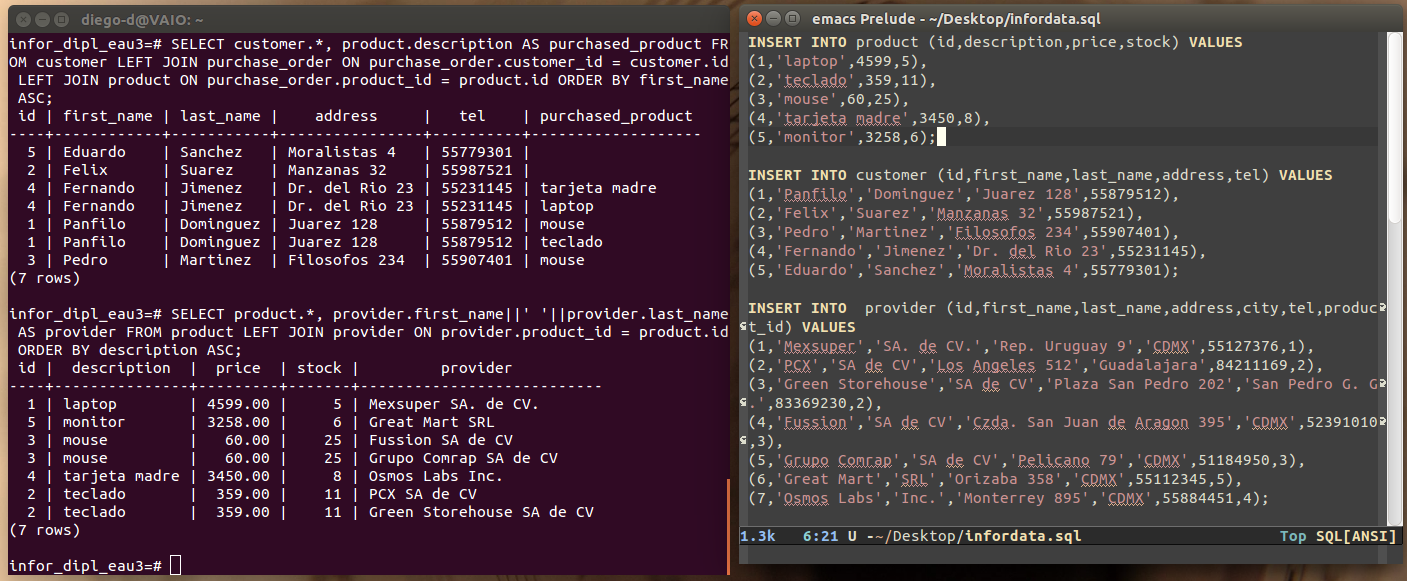
\includegraphics[width=1\textwidth]{./productproviders}~\\[1cm] 
	\end{center}	
	
	\subsection{Organizador físico}
	Si se toma por hecho que la empresa es pequeña, no requiere mayor requerimiento que almacenamiento simple en 3 SSD de 1.2TB a 500 MB/s de transferencia montados en un servidor con 16 GB de RAM.  
	
	\section{Conclusiones}
	Es importante tener conocimiento acerca del diseño de bases de datos para poder crear estructuras de datos eficientes que sirvan para tener la información necesaria que requiere el cliente y hacer mas rápida y concreta la consulta y escritura de estos datos, permitiendo la disponibilidad de un sistema con capa de persistencia confiable.
	
	
	\pagebreak
	\begin{thebibliography}{9}	
	
	\bibitem{psqldocs} The PostgreSQL Development Team. 
		\emph{PostgreSQL 7.0 Docs}. PostgreSQL, [Disponible en: http://www.postgresql.org/docs/7.0/static/postgres.htm].
	
		\bibitem{rrhopkins} Robert J. Robbins. 
		\emph{Database Fundamentals}. Johns Hopkins University, [Disponible en: http://www.esp.org/db-fund.pdf].
		
		\bibitem{elmasriynavathe} Ramez Elmasri and Shamkant Navathe. 
		\emph{Fundamentals of Database Systems}. Pearson Education, [Disponible en: http://tinman.cs.gsu.edu/~raj/4710/f11/Ch01.pdf].

	\end{thebibliography}

\end{document}
